\documentclass[11pt,ignorenonframetext,]{beamer}
\setbeamertemplate{caption}[numbered]
\setbeamertemplate{caption label separator}{: }
\setbeamercolor{caption name}{fg=normal text.fg}
\beamertemplatenavigationsymbolsempty
\usepackage{lmodern}
\usepackage{amssymb,amsmath}
\usepackage{ifxetex,ifluatex}
\usepackage{fixltx2e} % provides \textsubscript
\ifnum 0\ifxetex 1\fi\ifluatex 1\fi=0 % if pdftex
  \usepackage[T1]{fontenc}
  \usepackage[utf8]{inputenc}
\else % if luatex or xelatex
  \ifxetex
    \usepackage{mathspec}
  \else
    \usepackage{fontspec}
  \fi
  \defaultfontfeatures{Ligatures=TeX,Scale=MatchLowercase}
\fi
\usetheme[]{metropolis}
% use upquote if available, for straight quotes in verbatim environments
\IfFileExists{upquote.sty}{\usepackage{upquote}}{}
% use microtype if available
\IfFileExists{microtype.sty}{%
\usepackage{microtype}
\UseMicrotypeSet[protrusion]{basicmath} % disable protrusion for tt fonts
}{}
\newif\ifbibliography
\hypersetup{
            pdftitle={Lecture 2},
            pdfauthor={Colin Rundel},
            pdfborder={0 0 0},
            breaklinks=true}
\usepackage{color}
\usepackage{fancyvrb}
\newcommand{\VerbBar}{|}
\newcommand{\VERB}{\Verb[commandchars=\\\{\}]}
\DefineVerbatimEnvironment{Highlighting}{Verbatim}{commandchars=\\\{\}}
% Add ',fontsize=\small' for more characters per line
\newenvironment{Shaded}{}{}
\newcommand{\KeywordTok}[1]{\textcolor[rgb]{0.00,0.44,0.13}{\textbf{{#1}}}}
\newcommand{\DataTypeTok}[1]{\textcolor[rgb]{0.56,0.13,0.00}{{#1}}}
\newcommand{\DecValTok}[1]{\textcolor[rgb]{0.25,0.63,0.44}{{#1}}}
\newcommand{\BaseNTok}[1]{\textcolor[rgb]{0.25,0.63,0.44}{{#1}}}
\newcommand{\FloatTok}[1]{\textcolor[rgb]{0.25,0.63,0.44}{{#1}}}
\newcommand{\ConstantTok}[1]{\textcolor[rgb]{0.53,0.00,0.00}{{#1}}}
\newcommand{\CharTok}[1]{\textcolor[rgb]{0.25,0.44,0.63}{{#1}}}
\newcommand{\SpecialCharTok}[1]{\textcolor[rgb]{0.25,0.44,0.63}{{#1}}}
\newcommand{\StringTok}[1]{\textcolor[rgb]{0.25,0.44,0.63}{{#1}}}
\newcommand{\VerbatimStringTok}[1]{\textcolor[rgb]{0.25,0.44,0.63}{{#1}}}
\newcommand{\SpecialStringTok}[1]{\textcolor[rgb]{0.73,0.40,0.53}{{#1}}}
\newcommand{\ImportTok}[1]{{#1}}
\newcommand{\CommentTok}[1]{\textcolor[rgb]{0.38,0.63,0.69}{\textit{{#1}}}}
\newcommand{\DocumentationTok}[1]{\textcolor[rgb]{0.73,0.13,0.13}{\textit{{#1}}}}
\newcommand{\AnnotationTok}[1]{\textcolor[rgb]{0.38,0.63,0.69}{\textbf{\textit{{#1}}}}}
\newcommand{\CommentVarTok}[1]{\textcolor[rgb]{0.38,0.63,0.69}{\textbf{\textit{{#1}}}}}
\newcommand{\OtherTok}[1]{\textcolor[rgb]{0.00,0.44,0.13}{{#1}}}
\newcommand{\FunctionTok}[1]{\textcolor[rgb]{0.02,0.16,0.49}{{#1}}}
\newcommand{\VariableTok}[1]{\textcolor[rgb]{0.10,0.09,0.49}{{#1}}}
\newcommand{\ControlFlowTok}[1]{\textcolor[rgb]{0.00,0.44,0.13}{\textbf{{#1}}}}
\newcommand{\OperatorTok}[1]{\textcolor[rgb]{0.40,0.40,0.40}{{#1}}}
\newcommand{\BuiltInTok}[1]{{#1}}
\newcommand{\ExtensionTok}[1]{{#1}}
\newcommand{\PreprocessorTok}[1]{\textcolor[rgb]{0.74,0.48,0.00}{{#1}}}
\newcommand{\AttributeTok}[1]{\textcolor[rgb]{0.49,0.56,0.16}{{#1}}}
\newcommand{\RegionMarkerTok}[1]{{#1}}
\newcommand{\InformationTok}[1]{\textcolor[rgb]{0.38,0.63,0.69}{\textbf{\textit{{#1}}}}}
\newcommand{\WarningTok}[1]{\textcolor[rgb]{0.38,0.63,0.69}{\textbf{\textit{{#1}}}}}
\newcommand{\AlertTok}[1]{\textcolor[rgb]{1.00,0.00,0.00}{\textbf{{#1}}}}
\newcommand{\ErrorTok}[1]{\textcolor[rgb]{1.00,0.00,0.00}{\textbf{{#1}}}}
\newcommand{\NormalTok}[1]{{#1}}
\usepackage{graphicx,grffile}
\makeatletter
\def\maxwidth{\ifdim\Gin@nat@width>\linewidth\linewidth\else\Gin@nat@width\fi}
\def\maxheight{\ifdim\Gin@nat@height>\textheight0.8\textheight\else\Gin@nat@height\fi}
\makeatother
% Scale images if necessary, so that they will not overflow the page
% margins by default, and it is still possible to overwrite the defaults
% using explicit options in \includegraphics[width, height, ...]{}
\setkeys{Gin}{width=\maxwidth,height=\maxheight,keepaspectratio}

% Prevent slide breaks in the middle of a paragraph:
\widowpenalties 1 10000
\raggedbottom

\AtBeginPart{
  \let\insertpartnumber\relax
  \let\partname\relax
  \frame{\partpage}
}
\AtBeginSection{
  \ifbibliography
  \else
    \let\insertsectionnumber\relax
    \let\sectionname\relax
    \frame{\sectionpage}
  \fi
}
\AtBeginSubsection{
  \let\insertsubsectionnumber\relax
  \let\subsectionname\relax
  \frame{\subsectionpage}
}

\setlength{\parindent}{0pt}
\setlength{\parskip}{6pt plus 2pt minus 1pt}
\setlength{\emergencystretch}{3em}  % prevent overfull lines
\providecommand{\tightlist}{%
  \setlength{\itemsep}{0pt}\setlength{\parskip}{0pt}}
\setcounter{secnumdepth}{0}

\usepackage{geometry}
\usepackage{graphicx}
\usepackage{amssymb}
\usepackage{color}          	% gives color options
\usepackage{url}		% produces hyperlinks
\usepackage[english]{babel}
\usepackage{colortbl}	% allows for color usage in tables
\usepackage{multirow}	% allows for rows that span multiple rows in tables
\usepackage{xcolor}		% this package has a variety of color options
\usepackage{calc}
\usepackage{multicol}
\usepackage{wrapfig}
\usepackage{textcomp}
\usepackage{bm}
\usepackage{bbm}
\usepackage{setspace}
\singlespacing

%%%%%%%%%%%%%%%%
% Small code output
%%%%%%%%%%%%%%%%

%% change fontsize of R code
\let\oldShaded\Shaded
\let\endoldShaded\endShaded
\renewenvironment{Shaded}{\footnotesize\begin{spacing}{0.9}\oldShaded}{\endoldShaded\end{spacing}}

%% change fontsize of output
\let\oldverbatim\verbatim
\let\endoldverbatim\endverbatim
\renewenvironment{verbatim}{\footnotesize\begin{spacing}{0.9}\oldverbatim}{\endoldverbatim\end{spacing}}


%%%%%%%%%%%%%%%%
% Custom Colors
%%%%%%%%%%%%%%%%

\xdefinecolor{oiBlue}{rgb}{0.15, 0.35, 0.55}
\xdefinecolor{gray}{rgb}{0.5, 0.5, 0.5}
\xdefinecolor{darkGray}{rgb}{0.3, 0.3, 0.3}
\xdefinecolor{darkerGray}{rgb}{0.2, 0.2, 0.2}
\xdefinecolor{rubineRed}{rgb}{0.89,0,0.30}
\xdefinecolor{linkCol}{rgb}{0.11,0.49,0.95}	
\xdefinecolor{irishGreen}{rgb}{0,0.60,0}	
\xdefinecolor{darkturquoise}{rgb}{0.44, 0.58, 0.86}
\definecolor{lightGreen}{rgb}{0.533,0.765,0.42}
%\xdefinecolor{hlblue}{rgb}{0.051,0.65,1}
\xdefinecolor{hlblue}{rgb}{ 0.055, 0.639, 0.831}
\definecolor{light}{rgb}{.337,.608,.741}
\definecolor{dark}{rgb}{.337,.608,.741}

\definecolor{cpink}{rgb}{0.93, 0.23, 0.51}

%%%%%%%%%%%%%%%%
% Custom Commands
%%%%%%%%%%%%%%%%

% text colors
\newcommand{\red}[1]{\textit{\textcolor{rubineRed}{#1}}}
\newcommand{\orange}[1]{\textit{\textcolor{orange}{#1}}}
\newcommand{\pink}[1]{\textit{\textcolor{rubineRed!90!white!50}{#1}}}
\newcommand{\green}[1]{\textit{\textcolor{irishGreen}{#1}}}
\newcommand{\blue}[1]{\textit{\textcolor{darkturquoise}{#1}}}
\newcommand{\light}[1]{\textcolor{light}{\textbf{#1}}}
\newcommand{\dark}[1]{\textcolor{dark}{#1}}
\newcommand{\gray}[1]{\textcolor{gray}{#1}}


% links: webURL, webLin, appLink
\newcommand{\webURL}[1]{\urlstyle{same}{\textit{\textcolor{linkCol}{\url{#1}}} }}
\newcommand{\webLink}[2]{\href{#1}{\textcolor{linkCol}{{#2}}}}
\newcommand{\appLink}[2]{\href{#1}{\textcolor{lightGreen!80!black!90}{{#2}}}}

% mail
\newcommand{\mail}[1]{\href{mailto:#1}{\textit{\textcolor{linkCol}{#1}}}}

% highlighting: hl, hlGr, mathhl
\newcommand{\hl}[1]{\textit{\textcolor{hlblue}{#1}}}
\newcommand{\hlGr}[1]{\textit{\textcolor{lightGreen}{#1}}}
\newcommand{\hlRd}[1]{\textit{\textcolor{rubineRed}{#1}}}
\newcommand{\mathhl}[1]{\textcolor{hlblue}{\ensuremath{#1}}}

% example
\newcommand{\ex}[1]{\textcolor{blue}{{{\small (#1)}}}}


\DeclareMathOperator*{\argmin}{arg\,min}
\DeclareMathOperator*{\argmax}{arg\,max}

\title{Lecture 2}
\subtitle{Diagnostics and Model Evaluation}
\author{Colin Rundel}
\date{1/23/2017}

\begin{document}
\frame{\titlepage}

\section{From last time}\label{from-last-time}

\begin{frame}[fragile]{Linear model and data}

\begin{Shaded}
\begin{Highlighting}[]
\KeywordTok{library}\NormalTok{(rjags)}
\KeywordTok{library}\NormalTok{(dplyr)}

\KeywordTok{set.seed}\NormalTok{(}\DecValTok{01172017}\NormalTok{)}
\NormalTok{n =}\StringTok{ }\DecValTok{100}
\NormalTok{beta =}\StringTok{ }\KeywordTok{c}\NormalTok{(}\FloatTok{0.7}\NormalTok{,}\FloatTok{1.5}\NormalTok{,-}\FloatTok{2.2}\NormalTok{,}\FloatTok{0.1}\NormalTok{)}
\NormalTok{eps =}\StringTok{ }\KeywordTok{rnorm}\NormalTok{(n, }\DataTypeTok{mean=}\DecValTok{0}\NormalTok{, }\DataTypeTok{sd=}\DecValTok{1}\NormalTok{)}

\NormalTok{X0 =}\StringTok{ }\KeywordTok{rep}\NormalTok{(}\DecValTok{1}\NormalTok{, n)}
\NormalTok{X1 =}\StringTok{ }\KeywordTok{rt}\NormalTok{(n,}\DataTypeTok{df=}\DecValTok{5}\NormalTok{)}
\NormalTok{X2 =}\StringTok{ }\KeywordTok{rt}\NormalTok{(n,}\DataTypeTok{df=}\DecValTok{5}\NormalTok{)}
\NormalTok{X3 =}\StringTok{ }\KeywordTok{rt}\NormalTok{(n,}\DataTypeTok{df=}\DecValTok{5}\NormalTok{)}

\NormalTok{X =}\StringTok{ }\KeywordTok{cbind}\NormalTok{(X0, X1, X2, X3)}
\NormalTok{Y =}\StringTok{ }\NormalTok{X %*%}\StringTok{ }\NormalTok{beta +}\StringTok{ }\NormalTok{eps}
\NormalTok{d =}\StringTok{ }\KeywordTok{data.frame}\NormalTok{(Y,X[,-}\DecValTok{1}\NormalTok{]) }
\end{Highlighting}
\end{Shaded}

\end{frame}

\begin{frame}[fragile]{Bayesian model}

\begin{verbatim}
## model{
##   # Likelihood
##   for(i in 1:length(Y)){
##     Y[i]   ~ dnorm(mu[i],tau2)
##     mu[i] <- beta[1] + beta[2]*X1[i] + beta[3]*X2[i] + beta[4]*X3[i]
##   }
## 
##   # Prior for beta
##   for(j in 1:4){
##     beta[j] ~ dnorm(0,1/100)
##   }
## 
##   # Prior for the inverse variance
##   tau2   ~ dgamma(1, 1)
##   sigma <- 1/sqrt(tau2)
## }
\end{verbatim}

\end{frame}

\begin{frame}{}

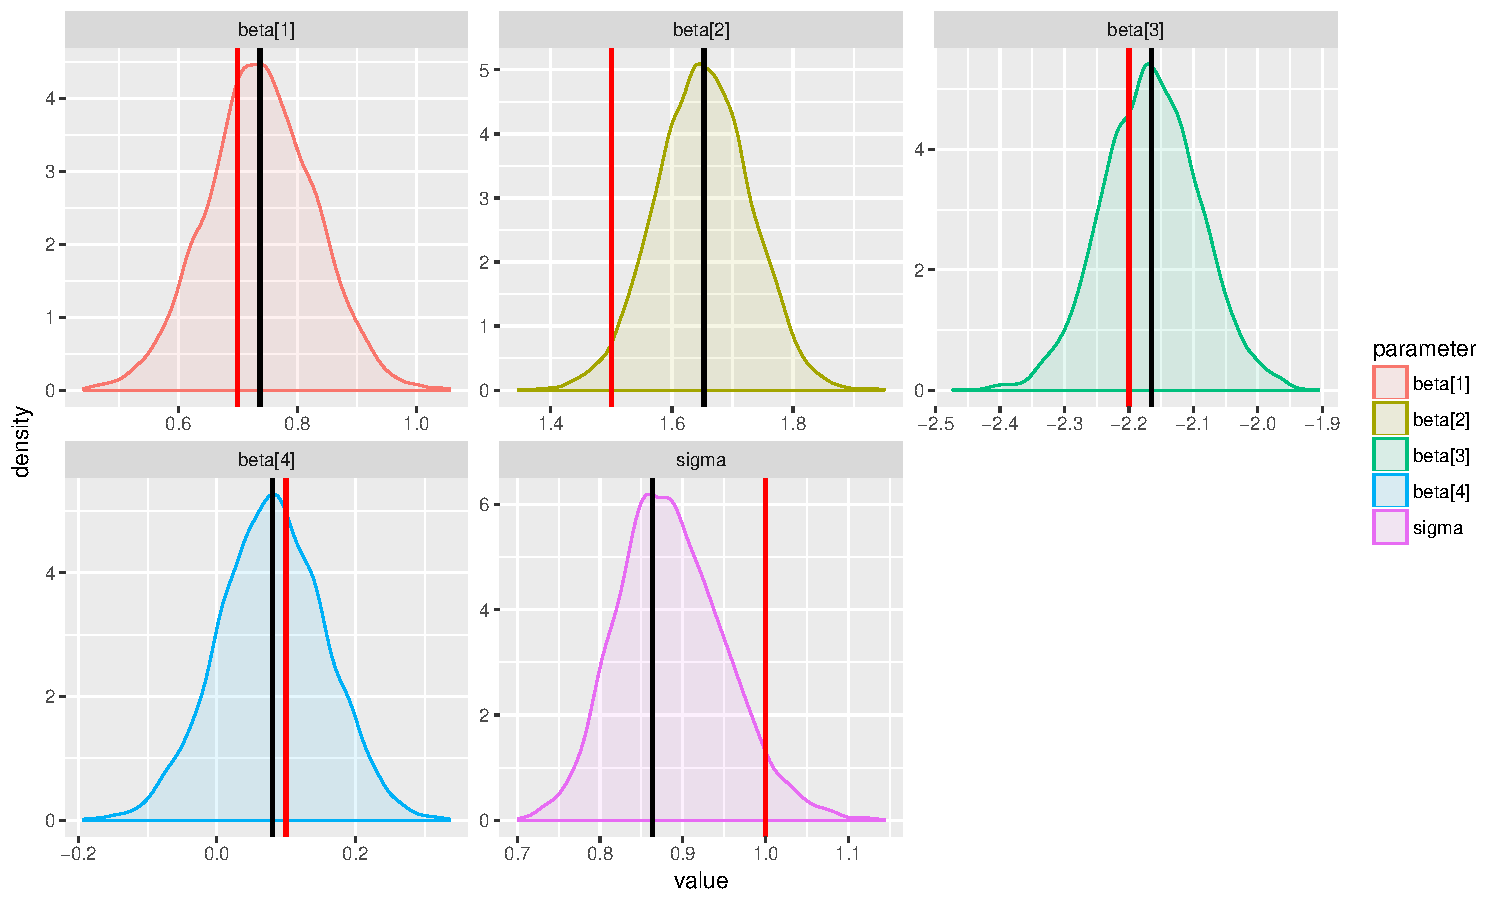
\includegraphics{Lec2_files/figure-beamer/unnamed-chunk-4-1.pdf}

\end{frame}

\section{Model Evaluation}\label{model-evaluation}

\begin{frame}{Model assessment?}

If we think back to our first regression class, one common option is
\(R^2\) which gives us the variability in \(Y\) explained by our model.

Quick review:

\pause

\[ \underset{\text{Total}}{\sum_{i}^n \left(Y_i - \bar{Y}\right)^2} = \underset{\text{Model}}{\sum_{i=1}^n \left(\hat{Y}_i - \bar{Y}\right)^2} + \underset{\text{Error }}{\sum_{i=1}^n \left(Y_i - \hat{Y}_i\right)^2} \]

\pause

\[ R^2 = \text{Corr}(\bm{Y}, \hat{\bm{Y}})^2 = \frac{\sum_{i=1}^n \left(\hat{Y}_i - \bar{Y}\right)^2}{\sum_{i=1}^n \left(Y_i - \bar{Y}\right)^2} = 1 - \frac{\sum_{i=1}^n \left(\hat{Y}_i - \hat{Y}_i\right)^2}{\sum_{i=1}^n \left(Y_i - \bar{Y}\right)^2}  \]

\end{frame}

\begin{frame}[fragile]{Bayesian \(R^2\)}

While we can collapse our posterior parameter distributions to a single
value (using mean, median, etc.) before calculating \(\hat{\bm{Y}}\) and
then \(R^2\), we don't need to.

\begin{Shaded}
\begin{Highlighting}[]
\NormalTok{n_sim =}\StringTok{ }\DecValTok{5000}\NormalTok{; n =}\StringTok{ }\DecValTok{100}
\NormalTok{Y_hat =}\StringTok{ }\KeywordTok{matrix}\NormalTok{(}\OtherTok{NA}\NormalTok{, }\DataTypeTok{nrow=}\NormalTok{n_sim, }\DataTypeTok{ncol=}\NormalTok{n, }\DataTypeTok{dimnames=}\KeywordTok{list}\NormalTok{(}\OtherTok{NULL}\NormalTok{, }\KeywordTok{paste0}\NormalTok{(}\StringTok{"Yhat["}\NormalTok{,}\DecValTok{1}\NormalTok{:n,}\StringTok{"]"}\NormalTok{)))}

\NormalTok{for(i in }\DecValTok{1}\NormalTok{:n_sim)}
\NormalTok{\{}
  \NormalTok{beta_post =}\StringTok{ }\NormalTok{samp[[}\DecValTok{1}\NormalTok{]][i,}\DecValTok{1}\NormalTok{:}\DecValTok{4}\NormalTok{]}
  \NormalTok{sigma_post =}\StringTok{ }\NormalTok{samp[[}\DecValTok{1}\NormalTok{]][i,}\DecValTok{5}\NormalTok{]}
  
  \NormalTok{Y_hat[i,] =}\StringTok{ }\NormalTok{beta_post %*%}\StringTok{ }\KeywordTok{t}\NormalTok{(X) +}\StringTok{ }\KeywordTok{rnorm}\NormalTok{(n, }\DataTypeTok{sd =} \NormalTok{sigma_post)}
\NormalTok{\}}

\NormalTok{Y_hat[}\DecValTok{1}\NormalTok{:}\DecValTok{5}\NormalTok{, }\DecValTok{1}\NormalTok{:}\DecValTok{5}\NormalTok{]}
\NormalTok{##         Yhat[1]  Yhat[2]   Yhat[3]    Yhat[4]    Yhat[5]}
\NormalTok{## [1,] -1.7193735 2.712832 -2.935192 -0.3472465 -0.5000324}
\NormalTok{## [2,]  0.4478495 3.035438 -4.419457  2.2174576  0.3661503}
\NormalTok{## [3,]  3.2258841 2.608588 -2.472159  1.1553329  1.7027229}
\NormalTok{## [4,]  1.8120911 2.612417 -3.349495  2.3028439  1.0398770}
\NormalTok{## [5,]  1.2504531 1.996477 -2.424596  0.5437237  0.7191012}
\end{Highlighting}
\end{Shaded}

\end{frame}

\begin{frame}{\(\hat{\bm{Y}}\) - lm vs Bayesian lm}

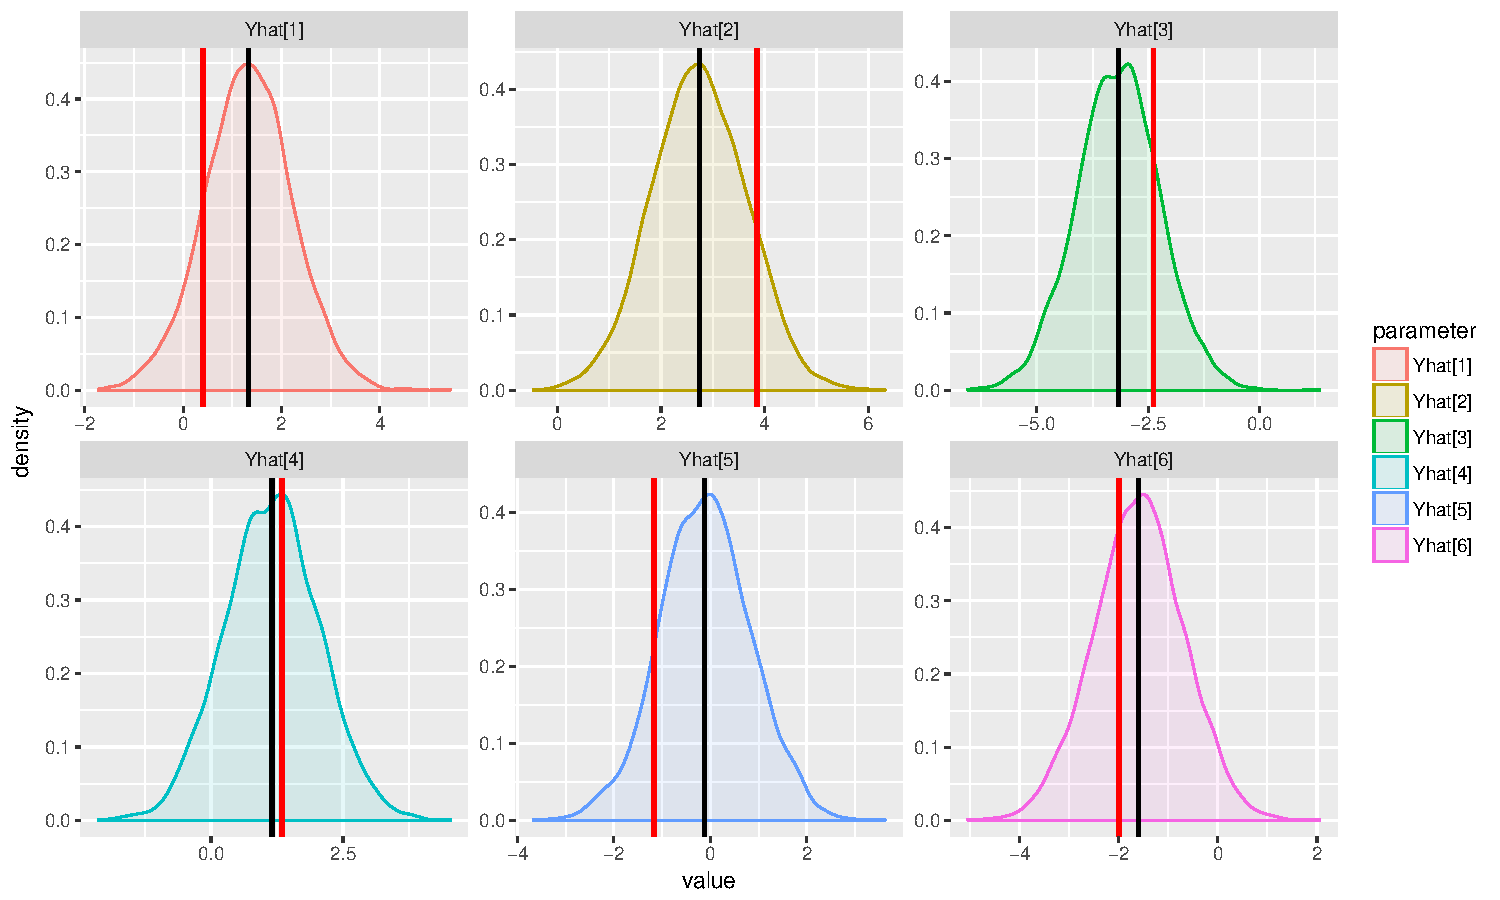
\includegraphics{Lec2_files/figure-beamer/unnamed-chunk-6-1.pdf}

\end{frame}

\begin{frame}[fragile]{Posterior \(R^2\)}

For each posterior sample \(s\) we can calculate
\(R^2_s = \text{Corr}(\bm{Y}, \hat{\bm{Y}}_s)^2\),

\begin{Shaded}
\begin{Highlighting}[]
\NormalTok{R2_post =}\StringTok{ }\KeywordTok{apply}\NormalTok{(Y_hat, }\DecValTok{1}\NormalTok{, function(Y_hat_s) }\KeywordTok{cor}\NormalTok{(Y, Y_hat_s)^}\DecValTok{2}\NormalTok{)}

\KeywordTok{summary}\NormalTok{(}\KeywordTok{c}\NormalTok{(R2_post)) %>%}\StringTok{ }\KeywordTok{t}\NormalTok{()}
\NormalTok{##        Min. 1st Qu. Median   Mean 3rd Qu.   Max.}
\NormalTok{## [1,] 0.7531  0.8410 0.8549 0.8536  0.8672 0.9168}

\KeywordTok{summary}\NormalTok{(}\KeywordTok{lm}\NormalTok{(Y~., }\DataTypeTok{data=}\NormalTok{d))$r.squared}
\NormalTok{## [1] 0.9262839}
\end{Highlighting}
\end{Shaded}

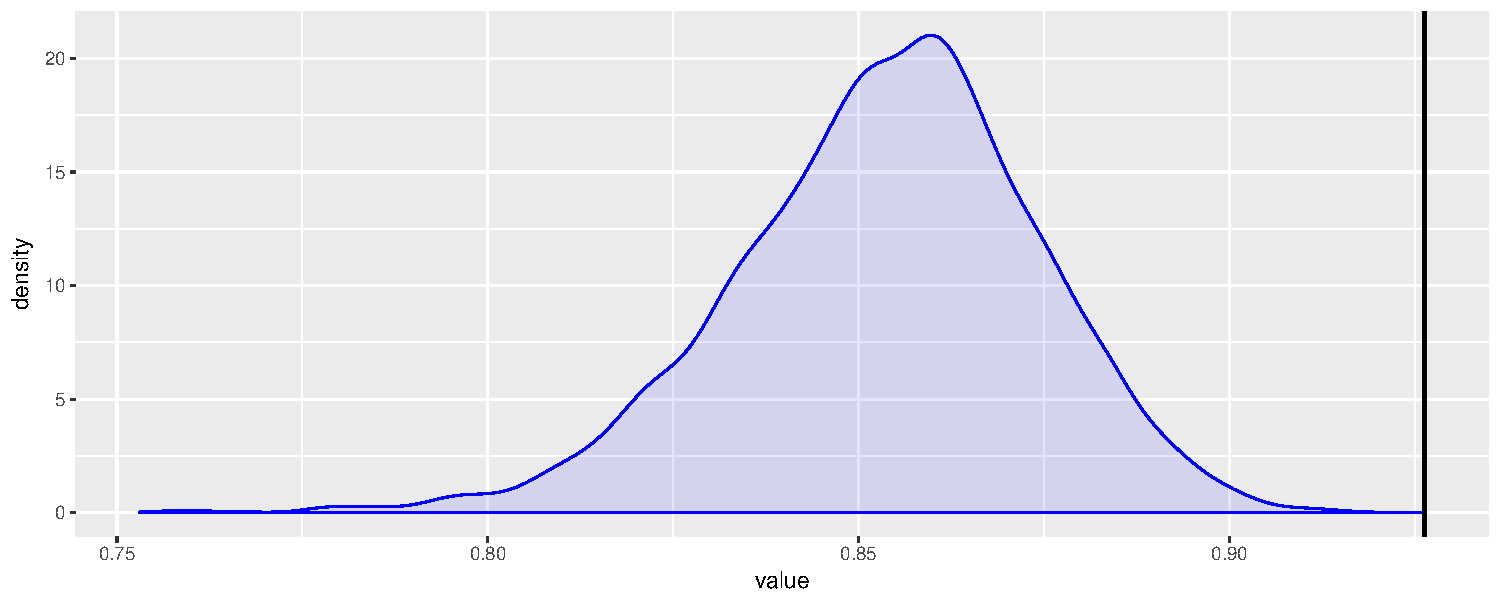
\includegraphics{Lec2_files/figure-beamer/unnamed-chunk-8-1.pdf}

\end{frame}

\begin{frame}[fragile]{What if we collapsed first?}

\begin{Shaded}
\begin{Highlighting}[]
\NormalTok{Y_hat_post_mean =}\StringTok{ }\KeywordTok{apply}\NormalTok{(Y_hat, }\DecValTok{2}\NormalTok{, mean) }
\KeywordTok{head}\NormalTok{(Y_hat_post_mean)}
\NormalTok{##    Yhat[1]    Yhat[2]    Yhat[3]    Yhat[4]    Yhat[5]    Yhat[6] }
\NormalTok{##  1.3324163  2.7363221 -3.1772690  1.1531411 -0.1029881 -1.5918980}

\NormalTok{Y_hat_post_med  =}\StringTok{ }\KeywordTok{apply}\NormalTok{(Y_hat, }\DecValTok{2}\NormalTok{, median) }
\KeywordTok{head}\NormalTok{(Y_hat_post_med)}
\NormalTok{##    Yhat[1]    Yhat[2]    Yhat[3]    Yhat[4]    Yhat[5]    Yhat[6] }
\NormalTok{##  1.3336394  2.7270929 -3.1659989  1.1631532 -0.1003662 -1.5807078}

\KeywordTok{cor}\NormalTok{(Y_hat_post_mean, Y)^}\DecValTok{2}
\NormalTok{##           [,1]}
\NormalTok{## [1,] 0.9264776}

\KeywordTok{cor}\NormalTok{(Y_hat_post_med,  Y)^}\DecValTok{2}
\NormalTok{##           [,1]}
\NormalTok{## [1,] 0.9264527}

\KeywordTok{summary}\NormalTok{(}\KeywordTok{lm}\NormalTok{(Y~., }\DataTypeTok{data=}\NormalTok{d))$r.squared}
\NormalTok{## [1] 0.9262839}
\end{Highlighting}
\end{Shaded}

\end{frame}

\begin{frame}{What went wrong?}

If our criteria is to maximize \(R^2\), then nothing. Why this result?

\pause

\(~\)

Remember that \(\hat{\beta}_{MLE} = \hat{\beta}_{LS}\), the latter of
which is achieved by

\[ \underset{\bm{\beta}}{\argmin} \sum_{i=1}^n \left( Y_i - \bm{X}_{i\cdot} \bm{\beta} \right)^2  = \underset{\bm{\beta}}{\argmin} \sum_{i=1}^n \left( Y_i - \hat{Y}_i \right)^2\]

\pause

\(~\)

So if we have \(\bm\beta\) such that it minimizes the least squares
criterion what does that tell us about

\[ R^2 = \text{Corr}(\bm{Y}, \hat{\bm{Y}})^2 = \frac{\sum_{i=1}^n \left(\hat{Y}_i - \bar{Y}\right)^2}{\sum_{i=1}^n \left(Y_i - \bar{Y}\right)^2} = 1 - \frac{\sum_{i=1}^n \left(Y_i - \hat{Y}_i\right)^2}{\sum_{i=1}^n \left(Y_i - \bar{Y}\right)^2}  \]

\end{frame}

\begin{frame}{Some problems with \(R^2\)}

\begin{itemize}
\item $R^2$ always increases (or stays the same) when a predictor is added  \\ ~\\
\item $R^2$ is highly susecptible to over fitting \\ ~\\
\item $R^2$ is sensitive to outliers \\ ~\\
\item $R^2$ depends heavily on current values of $Y$ \\ ~\\
\item $R^2$ can differ drastically for two equivalent models (i.e. nearly identical inferences about key parameters)
\end{itemize}

\end{frame}

\section{Other Metrics}\label{other-metrics}

\begin{frame}{Root Mean Square Error}

The traditional definition of rmse is as follows

\[ \text{RMSE} = \sqrt{ \frac{1}{n} \sum_{i=1}^n \left(Y_i - \hat{Y_i} \right)^2 } \]

In the bayesian context where we have posterior samples from each
parameter / prediction of interest we can express this equation as

\[ \text{RMSE} = \sqrt{ \frac{1}{n \, n_s} \sum_{s=1}^{n_s} \sum_{i=1}^n \left(Y_i - \hat{Y}_{i,s} \right)^2 } \]
\(~\)

Note that as we just saw with \(R^2\) using the first definition with
\(\hat{Y}_{i} = \sum_{s=1}^{n_s}\hat{Y}_{i,s} / n\) does not necessarily
give the same result as the 2nd equation.

\end{frame}

\begin{frame}{Continuous Rank Probability Score}

RMSE (and related metrics like MAE) are not directly applicable to
probabilistic predictions since they require fixed values of
\(\hat{Y}_i\). We can generalize to a fully continuous case where
\(\hat{Y}\) is given by a predictive distribution using a Continuous
Rank Probability Score

\[ \text{CRPS} = \int_{-\infty}^\infty \left(F_{\hat{Y}}(z) - \bm{1}_{\{z \geq Y\}}\right)^2 dz \]

where \(F_{\hat{Y}}\) is the empirical CDF of \(\hat{Y}\) (the posterior
predictive distribution for \(Y\)) and \(\bm{1}_{z \geq Y}\) is the
indicator function which equals 1 when \(z \geq Y\), the true/observed
value of \(Y\).

\end{frame}

\begin{frame}{Accuracy vs.~Precision}

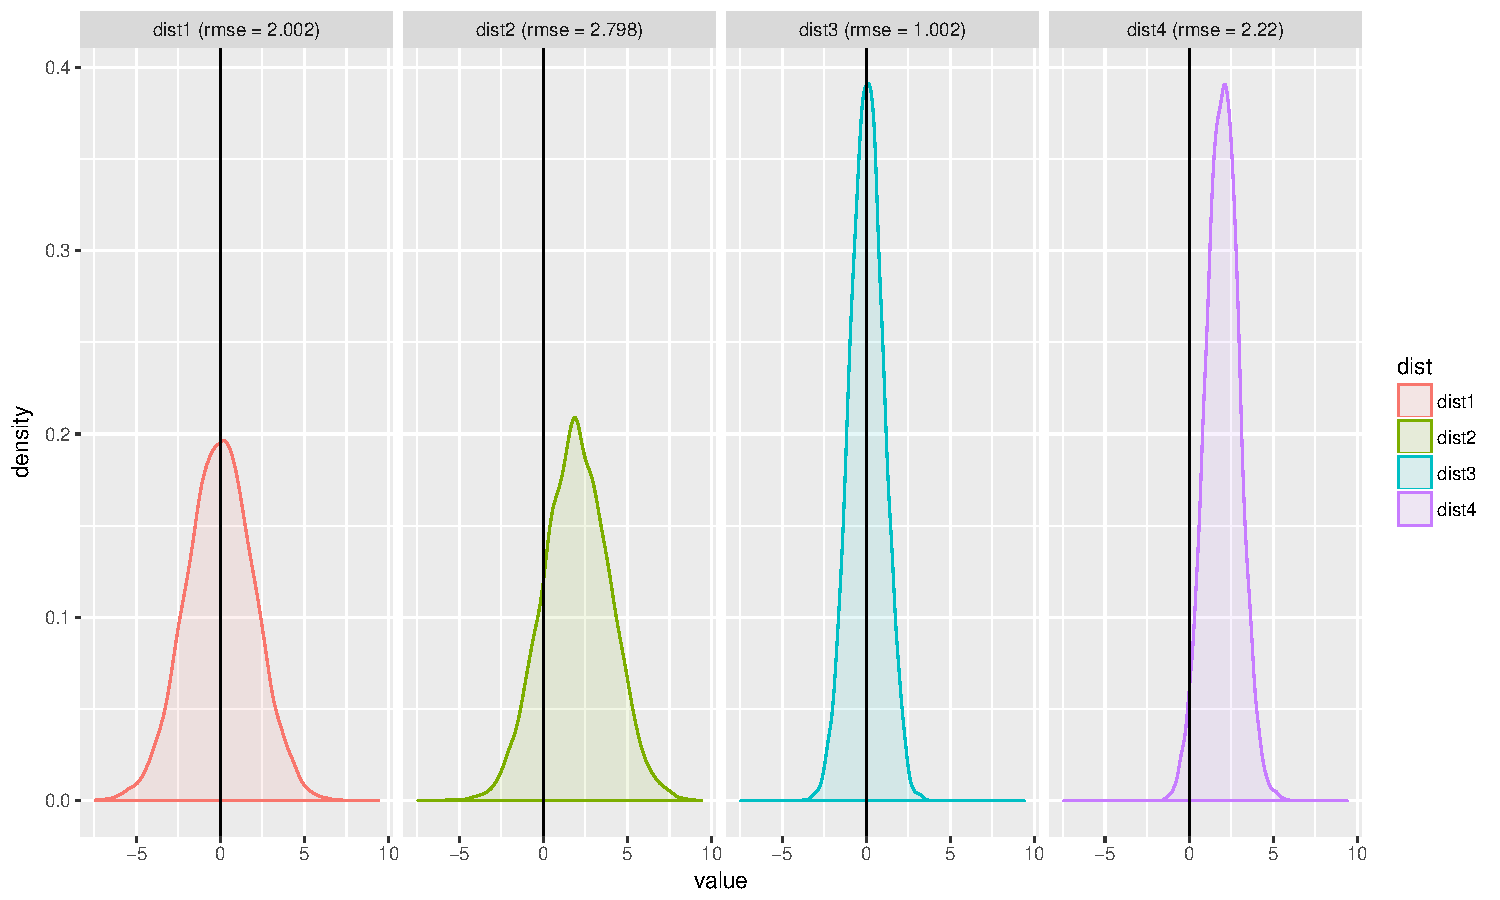
\includegraphics{Lec2_files/figure-beamer/unnamed-chunk-10-1.pdf}

\end{frame}

\begin{frame}[fragile]{CDF vs Indicator}

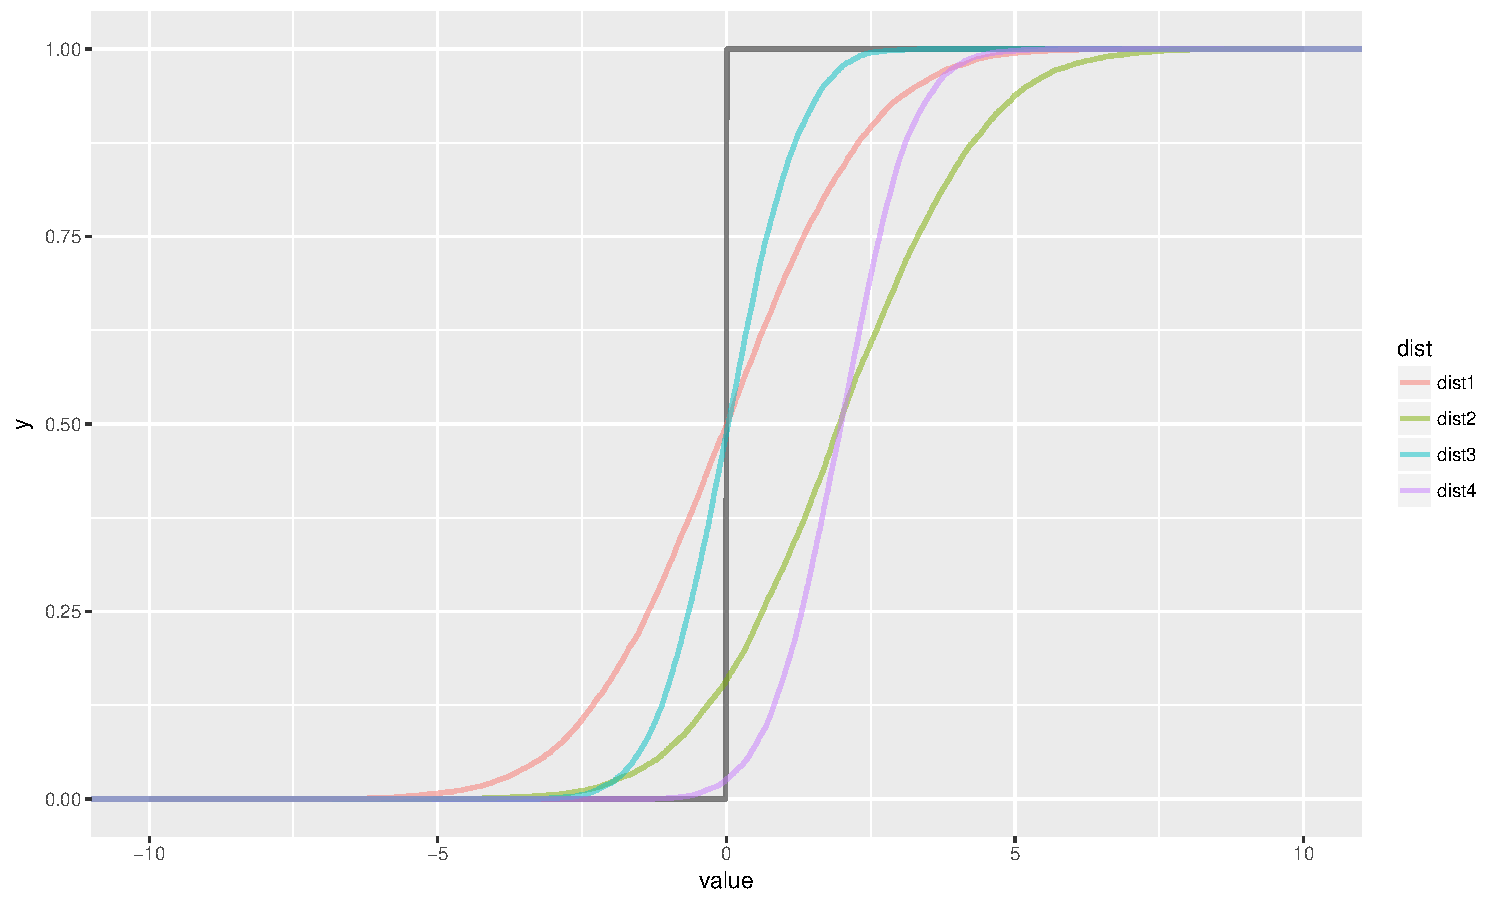
\includegraphics{Lec2_files/figure-beamer/unnamed-chunk-11-1.pdf}

\begin{verbatim}
## dist1 dist2 dist3 dist4 
## 0.468 1.188 0.235 1.432
\end{verbatim}

\end{frame}

\begin{frame}[fragile]{Empirical Coverage}

One final method of assessing model calibration is assessing how well
credible intervals, derived from the posterior predictive distributions
of the \(Y\)s, capture the true/observed values.

\pause

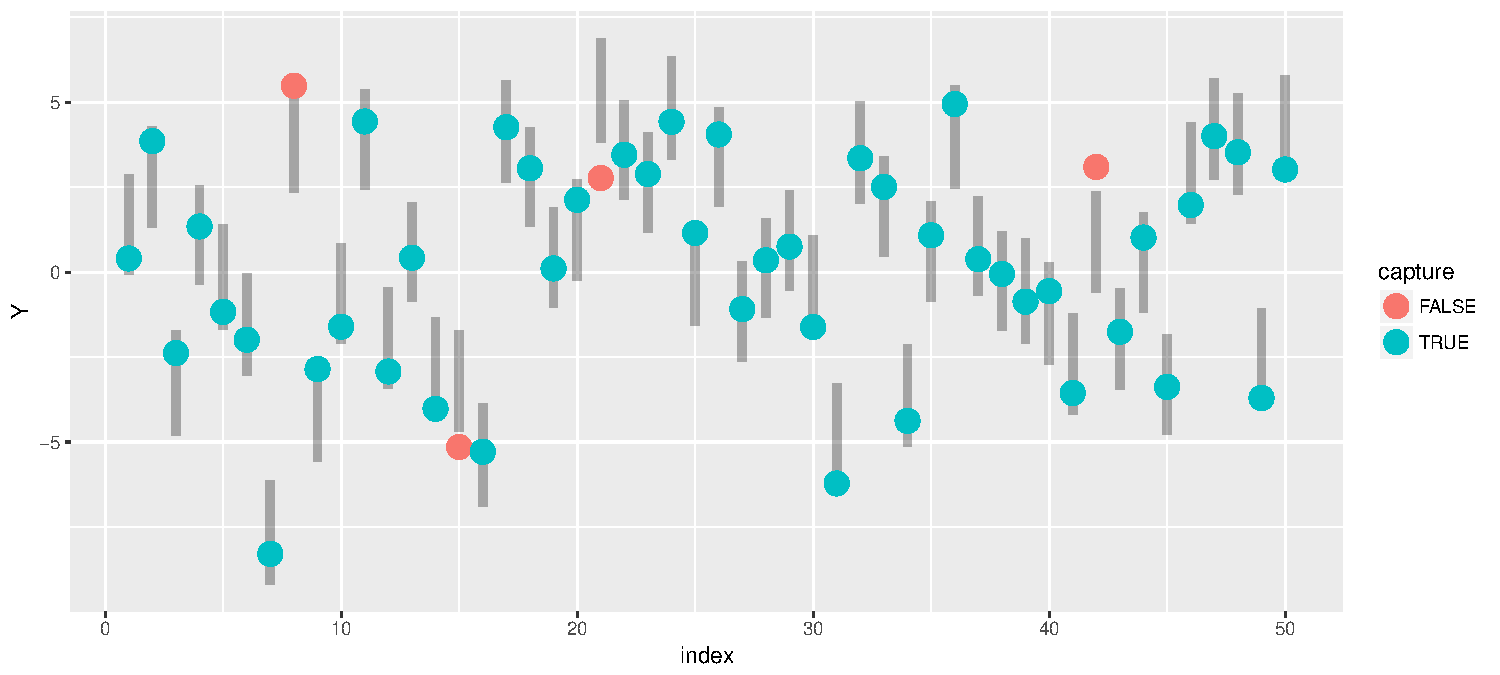
\includegraphics{Lec2_files/figure-beamer/unnamed-chunk-12-1.pdf}

\begin{verbatim}
## 90% CI empirical coverage 
##                      0.92
\end{verbatim}

\end{frame}

\section{Cross-validation}\label{cross-validation}

\begin{frame}{Cross-validation styles}

Kaggle style:

\begin{center}
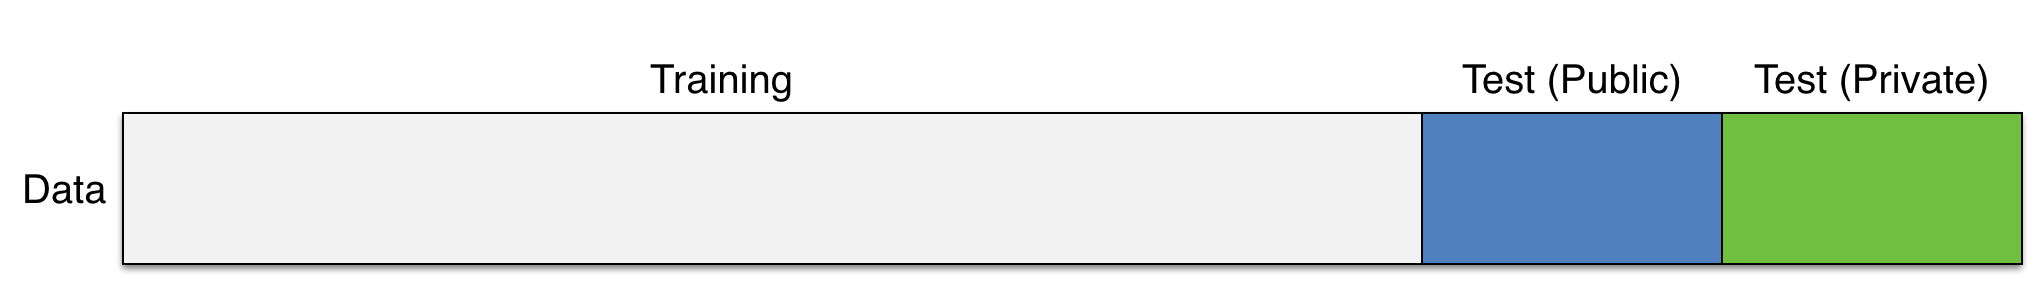
\includegraphics[width=0.8\textwidth]{figs/kaggle.png}
\end{center}

\(k\)-fold:

\begin{center}
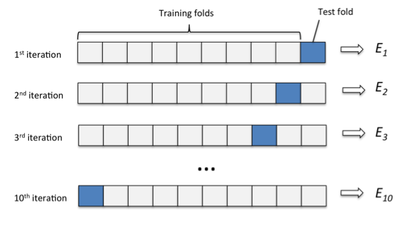
\includegraphics[width=0.8\textwidth]{figs/k-fold.png}
\end{center}

\end{frame}

\begin{frame}[fragile]{Cross-validation in R with \texttt{modelr}}

\begin{Shaded}
\begin{Highlighting}[]
\KeywordTok{library}\NormalTok{(modelr)}

\NormalTok{d_kaggle =}\StringTok{ }\KeywordTok{resample_partition}\NormalTok{(d, }\KeywordTok{c}\NormalTok{(}\DataTypeTok{train=}\FloatTok{0.70}\NormalTok{, }\DataTypeTok{test1=}\FloatTok{0.15}\NormalTok{, }\DataTypeTok{test2=}\FloatTok{0.15}\NormalTok{))}
\NormalTok{d_kaggle}
\NormalTok{## $train}
\NormalTok{## <resample [69 x 4]> 1, 2, 3, 4, 6, 7, 8, 9, 11, 13, ...}
\NormalTok{## }
\NormalTok{## $test1}
\NormalTok{## <resample [15 x 4]> 12, 19, 23, 30, 34, 35, 36, 48, 54, 58, ...}
\NormalTok{## }
\NormalTok{## $test2}
\NormalTok{## <resample [16 x 4]> 5, 10, 18, 21, 31, 41, 45, 46, 57, 68, ...}

\NormalTok{d_kfold =}\StringTok{ }\KeywordTok{crossv_kfold}\NormalTok{(d, }\DataTypeTok{k=}\DecValTok{5}\NormalTok{)}
\NormalTok{d_kfold}
\NormalTok{## # A tibble: 5 × 3}
\NormalTok{##            train           test   .id}
\NormalTok{##           <list>         <list> <chr>}
\NormalTok{## 1 <S3: resample> <S3: resample>     1}
\NormalTok{## 2 <S3: resample> <S3: resample>     2}
\NormalTok{## 3 <S3: resample> <S3: resample>     3}
\NormalTok{## 4 <S3: resample> <S3: resample>     4}
\NormalTok{## 5 <S3: resample> <S3: resample>     5}
\end{Highlighting}
\end{Shaded}

\end{frame}

\begin{frame}[fragile]{\texttt{resample} objects}

The simple idea behind \texttt{resample} objects is that there is no
need to create and hold on to these subsets / partitions of the original
data frame - only need to track which rows belong to what subset and
then handle the creation of the new data frame when necessary.

\begin{Shaded}
\begin{Highlighting}[]
\NormalTok{d_kaggle$test1}
\NormalTok{## <resample [15 x 4]> 12, 19, 23, 30, 34, 35, 36, 48, 54, 58, ...}

\KeywordTok{str}\NormalTok{(d_kaggle$test1)}
\NormalTok{## List of 2}
\NormalTok{##  $ data:'data.frame':    100 obs. of  4 variables:}
\NormalTok{##   ..$ Y : num [1:100] 0.402 3.855 -2.384 1.344 -1.171 ...}
\NormalTok{##   ..$ X1: num [1:100] 0.0513 0.0259 -1.2622 -0.443 -3.1655 ...}
\NormalTok{##   ..$ X2: num [1:100] -0.284 -0.928 0.948 -0.535 -1.961 ...}
\NormalTok{##   ..$ X3: num [1:100] -1.279 -0.571 2.938 -0.15 1.664 ...}
\NormalTok{##  $ idx : int [1:15] 12 19 23 30 34 35 36 48 54 58 ...}
\NormalTok{##  - attr(*, "class")= chr "resample"}

\KeywordTok{as.data.frame}\NormalTok{(d_kaggle$test1)}
\NormalTok{##             Y          X1         X2          X3}
\NormalTok{## 12 -2.9263300 -0.82679975  0.5995159 -1.64750639}
\NormalTok{## 19  0.1090239  1.34327879  1.1326438 -0.16019583}
\NormalTok{## 23  2.8883752  0.40828680 -0.5064750  1.58942370}
\NormalTok{## 30 -1.6175504  0.36906392  0.8140513  1.09849733}
\NormalTok{## 34 -4.3808207 -0.92931006  1.2761635 -0.07280222}
\NormalTok{## 35  1.0838832 -1.14245830 -0.8071982 -0.42909876}
\NormalTok{## 36  4.9475852  1.23069336 -0.5259891  1.24623765}
\NormalTok{## 48  3.5253998 -0.03160771 -1.4007319  0.33505032}
\NormalTok{## 54  2.5509245  0.55451423  0.6706189 -1.23927415}
\NormalTok{## 58 -5.5803991 -2.85497337  0.3868060 -0.59530294}
\NormalTok{## 61  1.1533307  0.18753117  0.3792767 -0.51489211}
\NormalTok{## 75  3.2602915 -0.26286979 -1.0864605 -0.80689652}
\NormalTok{## 77  4.0306491  0.36510853 -1.2046542 -0.71226369}
\NormalTok{## 79 -1.1785578 -0.76090999 -0.4101772 -1.53249336}
\NormalTok{## 88 -4.8509066 -2.90893682  1.1153282 -0.61301759}
\end{Highlighting}
\end{Shaded}

\end{frame}

\begin{frame}[fragile]{Simple usage}

\begin{Shaded}
\begin{Highlighting}[]
\NormalTok{lm_train =}\StringTok{ }\KeywordTok{lm}\NormalTok{(Y~., }\DataTypeTok{data=}\NormalTok{d_kaggle$train)}
 
\NormalTok{lm_train %>%}\StringTok{ }\KeywordTok{summary}\NormalTok{() %$%}\StringTok{ }\NormalTok{r.squared}
\NormalTok{## [1] 0.9410859}

\KeywordTok{rsquare}\NormalTok{(lm_train, d_kaggle$train)}
\NormalTok{## [1] 0.9410859}


\NormalTok{Y_hat_test1 =}\StringTok{ }\KeywordTok{predict}\NormalTok{(lm_train, d_kaggle$test1)}

\NormalTok{(Y_hat_test1 -}\StringTok{ }\KeywordTok{as.data.frame}\NormalTok{(d_kaggle$test1)$Y)^}\DecValTok{2} \NormalTok\StringTok{ }\KeywordTok{mean}\NormalTok{() %>%}\StringTok{ }\KeywordTok{sqrt}\NormalTok{()}
\NormalTok{## [1] 1.071201}

\KeywordTok{rmse}\NormalTok{(lm_train, d_kaggle$test1)}
\NormalTok{## [1] 1.071201}

\KeywordTok{rmse}\NormalTok{(lm_train, d_kaggle$test2)}
\NormalTok{## [1] 1.031323}
\end{Highlighting}
\end{Shaded}

\end{frame}

\begin{frame}[fragile]{Aside: \texttt{purrr}}

\texttt{purrr} is a package by Hadley which improves functional
programming in R by focusing on pure and type stable functions. It
provides basic functions for looping over objects and returning a value
(of a specific type) - think of it as a better version of
\texttt{lapply}/\texttt{sapply}/\texttt{vapply}.

\begin{itemize}
\item
  \texttt{map()} - returns a list.
\item
  \texttt{map\_lgl()} - returns a logical vector.
\item
  \texttt{map\_int()} - returns a integer vector.
\item
  \texttt{map\_dbl()} - returns a double vector.
\item
  \texttt{map\_chr()} - returns a character vector.
\item
  \texttt{map\_df()} - returns a data frame.
\item
  \texttt{map2\_*} - variants for iterating over two vectors
  simultaneously.
\end{itemize}

\end{frame}

\begin{frame}[fragile]{Aside: Type Consistency}

R is a weakly / dynamically typed language which means there is no way
to define a function which enforces the argument or return types.

This flexibility can be useful at times, but often it makes it hard to
reason about your code and requires more verbose code to handle edge
cases.

\begin{Shaded}
\begin{Highlighting}[]
\KeywordTok{library}\NormalTok{(purrr)}
\NormalTok{## }
\NormalTok{## Attaching package: 'purrr'}
\NormalTok{## The following objects are masked from 'package:dplyr':}
\NormalTok{## }
\NormalTok{##     contains, order_by}
\NormalTok{## The following object is masked from 'package:magrittr':}
\NormalTok{## }
\NormalTok{##     set_names}

\KeywordTok{map_dbl}\NormalTok{(}\KeywordTok{list}\NormalTok{(}\KeywordTok{rnorm}\NormalTok{(}\FloatTok{1e3}\NormalTok{),}\KeywordTok{rnorm}\NormalTok{(}\FloatTok{1e3}\NormalTok{),}\KeywordTok{rnorm}\NormalTok{(}\FloatTok{1e3}\NormalTok{)), mean)}
\NormalTok{## [1] -0.02679155  0.02086224 -0.01229868}
\KeywordTok{map_chr}\NormalTok{(}\KeywordTok{list}\NormalTok{(}\KeywordTok{rnorm}\NormalTok{(}\FloatTok{1e3}\NormalTok{),}\KeywordTok{rnorm}\NormalTok{(}\FloatTok{1e3}\NormalTok{),}\KeywordTok{rnorm}\NormalTok{(}\FloatTok{1e3}\NormalTok{)), mean)}
\NormalTok{## [1] "0.021504"  "0.025358"  "-0.035972"}
\KeywordTok{map_int}\NormalTok{(}\KeywordTok{list}\NormalTok{(}\KeywordTok{rnorm}\NormalTok{(}\FloatTok{1e3}\NormalTok{),}\KeywordTok{rnorm}\NormalTok{(}\FloatTok{1e3}\NormalTok{),}\KeywordTok{rnorm}\NormalTok{(}\FloatTok{1e3}\NormalTok{)), mean)}
\NormalTok{## Error: Can't coerce element 1 from a double to a integer}
\end{Highlighting}
\end{Shaded}

\end{frame}

\begin{frame}[fragile]{Aside: Anonymous Functions shortcut}

An anonymous function is one that is never given a name (i.e.~assigned
to a variable), using base R we would write something like the
following,

\begin{Shaded}
\begin{Highlighting}[]
\KeywordTok{sapply}\NormalTok{(}\DecValTok{1}\NormalTok{:}\DecValTok{10}\NormalTok{, function(x) x^(x}\DecValTok{+1}\NormalTok{))}
\NormalTok{##  [1]            1            8           81         1024        15625}
\NormalTok{##  [6]       279936      5764801    134217728   3486784401 100000000000}
\end{Highlighting}
\end{Shaded}

purrr lets us write anonymous functions using the traditional style, but
also lets us use one sided formulas where the value being mapped is
referenced by \texttt{.}

\begin{Shaded}
\begin{Highlighting}[]
\KeywordTok{map_dbl}\NormalTok{(}\DecValTok{1}\NormalTok{:}\DecValTok{10}\NormalTok{, function(x) x^(x}\DecValTok{+1}\NormalTok{))}
\NormalTok{##  [1]            1            8           81         1024        15625}
\NormalTok{##  [6]       279936      5764801    134217728   3486784401 100000000000}

\KeywordTok{map_dbl}\NormalTok{(}\DecValTok{1}\NormalTok{:}\DecValTok{10}\NormalTok{, ~}\StringTok{ }\NormalTok{.^(.+}\DecValTok{1}\NormalTok{))}
\NormalTok{##  [1]            1            8           81         1024        15625}
\NormalTok{##  [6]       279936      5764801    134217728   3486784401 100000000000}
\end{Highlighting}
\end{Shaded}

\end{frame}

\begin{frame}[fragile]{Cross-validation in R with \texttt{modelr} +
\texttt{purrr}}

\begin{Shaded}
\begin{Highlighting}[]
\NormalTok{lm_models =}\StringTok{ }\KeywordTok{map}\NormalTok{(d_kfold$train, ~}\StringTok{ }\KeywordTok{lm}\NormalTok{(Y~., }\DataTypeTok{data=}\NormalTok{.))}
\KeywordTok{str}\NormalTok{(lm_models, }\DataTypeTok{max.level =} \DecValTok{1}\NormalTok{)}
\NormalTok{## List of 5}
\NormalTok{##  $ 1:List of 12}
\NormalTok{##   ..- attr(*, "class")= chr "lm"}
\NormalTok{##  $ 2:List of 12}
\NormalTok{##   ..- attr(*, "class")= chr "lm"}
\NormalTok{##  $ 3:List of 12}
\NormalTok{##   ..- attr(*, "class")= chr "lm"}
\NormalTok{##  $ 4:List of 12}
\NormalTok{##   ..- attr(*, "class")= chr "lm"}
\NormalTok{##  $ 5:List of 12}
\NormalTok{##   ..- attr(*, "class")= chr "lm"}

\KeywordTok{map2_dbl}\NormalTok{(lm_models, d_kfold$train, rsquare)}
\NormalTok{##         1         2         3         4         5 }
\NormalTok{## 0.9201087 0.9137336 0.9285830 0.9379184 0.9301658}

\KeywordTok{map2_dbl}\NormalTok{(lm_models, d_kfold$test, rmse)}
\NormalTok{##         1         2         3         4         5 }
\NormalTok{## 0.8957795 0.6809255 0.8808314 1.0825899 0.8538277}
\end{Highlighting}
\end{Shaded}

\end{frame}

\begin{frame}[fragile]{Getting \texttt{modelr} to play nice with
\texttt{rjags}}

We used the following code to fit out model previously, lets generalize
/ functionalize it so we can use it with modelr

\begin{Shaded}
\begin{Highlighting}[]
\NormalTok{m =}\StringTok{ }\KeywordTok{jags.model}\NormalTok{(}
        \KeywordTok{textConnection}\NormalTok{(model), }
        \DataTypeTok{data =} \KeywordTok{list}\NormalTok{(}\DataTypeTok{Y=}\KeywordTok{c}\NormalTok{(Y), }\DataTypeTok{X1=}\NormalTok{X1, }\DataTypeTok{X2=}\NormalTok{X2, }\DataTypeTok{X3=}\NormalTok{X3)}
       \NormalTok{) }
\KeywordTok{update}\NormalTok{(m, }\DataTypeTok{n.iter=}\DecValTok{1000}\NormalTok{, }\DataTypeTok{progress.bar=}\StringTok{"none"}\NormalTok{)}
\NormalTok{samp =}\StringTok{ }\KeywordTok{coda.samples}\NormalTok{(}
        \NormalTok{m, }\DataTypeTok{variable.names=}\KeywordTok{c}\NormalTok{(}\StringTok{"beta"}\NormalTok{,}\StringTok{"sigma"}\NormalTok{), }
        \DataTypeTok{n.iter=}\DecValTok{5000}\NormalTok{, }\DataTypeTok{progress.bar=}\StringTok{"none"}
       \NormalTok{)}
\end{Highlighting}
\end{Shaded}

\end{frame}

\begin{frame}[fragile]{Fitting the model}

\begin{Shaded}
\begin{Highlighting}[]
\NormalTok{fit_jags_lm =}\StringTok{ }\NormalTok{function(data, }\DataTypeTok{n_burnin=}\DecValTok{1000}\NormalTok{, }\DataTypeTok{n_samps=}\DecValTok{5000}\NormalTok{)}
\NormalTok{\{}
  \NormalTok{data =}\StringTok{ }\KeywordTok{as.data.frame}\NormalTok{(data, }\DataTypeTok{optional=}\OtherTok{TRUE}\NormalTok{)}

  \NormalTok{m =}\StringTok{ }\KeywordTok{jags.model}\NormalTok{(}\KeywordTok{textConnection}\NormalTok{(model), }\DataTypeTok{data =} \NormalTok{data, }\DataTypeTok{quiet=}\OtherTok{TRUE}\NormalTok{)}
  \KeywordTok{update}\NormalTok{(m, }\DataTypeTok{n.iter=}\NormalTok{n_burnin, }\DataTypeTok{progress.bar=}\StringTok{"none"}\NormalTok{)}
  \KeywordTok{coda.samples}\NormalTok{(}
    \NormalTok{m, }\DataTypeTok{variable.names=}\KeywordTok{c}\NormalTok{(}\StringTok{"beta"}\NormalTok{,}\StringTok{"sigma"}\NormalTok{), }
    \DataTypeTok{n.iter=}\NormalTok{n_samps, }\DataTypeTok{progress.bar=}\StringTok{"none"}
  \NormalTok{)[[}\DecValTok{1}\NormalTok{]]}
\NormalTok{\}}
\end{Highlighting}
\end{Shaded}

\end{frame}

\begin{frame}[fragile]{Predicting the model}

\begin{Shaded}
\begin{Highlighting}[]
\NormalTok{predict_jags_lm =}\StringTok{ }\NormalTok{function(samp, newdata)}
\NormalTok{\{}
  \NormalTok{data =}\StringTok{ }\KeywordTok{as.data.frame}\NormalTok{(newdata, }\DataTypeTok{optional=}\OtherTok{TRUE}\NormalTok{) %>%}\StringTok{ }\KeywordTok{tbl_df}\NormalTok{()}
  
  \NormalTok{n =}\StringTok{ }\KeywordTok{nrow}\NormalTok{(newdata)}
  \NormalTok{beta0_post =}\StringTok{ }\NormalTok{samp[,}\DecValTok{1}\NormalTok{]; beta1_post =}\StringTok{ }\NormalTok{samp[,}\DecValTok{2}\NormalTok{]}
  \NormalTok{beta2_post =}\StringTok{ }\NormalTok{samp[,}\DecValTok{3}\NormalTok{]; beta3_post =}\StringTok{ }\NormalTok{samp[,}\DecValTok{4}\NormalTok{]}
  \NormalTok{sigma_post =}\StringTok{ }\NormalTok{samp[,}\DecValTok{5}\NormalTok{]}
  
  \NormalTok{data$post_pred =}\StringTok{ }\KeywordTok{list}\NormalTok{(}\OtherTok{NA}\NormalTok{)}
  \NormalTok{for(i in }\DecValTok{1}\NormalTok{:n)}
  \NormalTok{\{}
    \NormalTok{mu =}\StringTok{ }\NormalTok{beta0_post *}\StringTok{ }\DecValTok{1}          \NormalTok{+}\StringTok{ }\NormalTok{beta1_post *}\StringTok{ }\NormalTok{data$X1[i] +}\StringTok{ }
\StringTok{         }\NormalTok{beta2_post *}\StringTok{ }\NormalTok{data$X2[i] +}\StringTok{ }\NormalTok{beta3_post *}\StringTok{ }\NormalTok{data$X3[i] }
    \NormalTok{error =}\StringTok{ }\KeywordTok{rnorm}\NormalTok{(n_sim, }\DataTypeTok{sd =} \NormalTok{sigma_post)}
    
    \NormalTok{data$post_pred[[i]] =}\StringTok{ }\NormalTok{mu +}\StringTok{ }\NormalTok{error}
  \NormalTok{\}}
  
  \NormalTok{data}
\NormalTok{\}}
\end{Highlighting}
\end{Shaded}

\end{frame}

\begin{frame}[fragile]{Empirical Coverage}

\begin{Shaded}
\begin{Highlighting}[]
\NormalTok{empcov =}\StringTok{ }\NormalTok{function(pred, obs_col, }\DataTypeTok{width=}\FloatTok{0.9}\NormalTok{)}
\NormalTok{\{}
  \NormalTok{cred_int =}\StringTok{ }\KeywordTok{map}\NormalTok{(pred$post_pred, ~}\StringTok{ }\KeywordTok{HPDinterval}\NormalTok{(., width)) %>%}\StringTok{ }
\StringTok{    }\KeywordTok{do.call}\NormalTok{(rbind, .)}
  
  \NormalTok{observed =}\StringTok{ }\NormalTok{pred[[obs_col]]}
  
  \NormalTok{data =}\StringTok{ }\KeywordTok{cbind}\NormalTok{(pred, cred_int) %>%}\StringTok{ }
\StringTok{    }\KeywordTok{tbl_df}\NormalTok{() %>%}
\StringTok{    }\KeywordTok{mutate}\NormalTok{(}\DataTypeTok{capture =} \NormalTok{lower <=}\StringTok{ }\NormalTok{observed &}\StringTok{ }\NormalTok{upper >=}\StringTok{ }\NormalTok{observed)}
  
  \KeywordTok{cat}\NormalTok{(width*}\DecValTok{100}\NormalTok{,}\StringTok{"% CI empirical coverage = "}\NormalTok{, }
      \KeywordTok{round}\NormalTok{(}\KeywordTok{sum}\NormalTok{(data$capture)/}\KeywordTok{nrow}\NormalTok{(data),}\DecValTok{3}\NormalTok{), }\StringTok{"}\CharTok{\textbackslash{}n}\StringTok{"}\NormalTok{, }\DataTypeTok{sep=}\StringTok{""}\NormalTok{) }
  
  \KeywordTok{invisible}\NormalTok{(data)}
\NormalTok{\}}
\end{Highlighting}
\end{Shaded}

\end{frame}

\begin{frame}[fragile]{Putting it together}

\begin{Shaded}
\begin{Highlighting}[]
\NormalTok{model_fit =}\StringTok{ }\KeywordTok{fit_jags_lm}\NormalTok{(d_kaggle$train)}
\NormalTok{train_pred =}\StringTok{ }\KeywordTok{predict_jags_lm}\NormalTok{(model_fit, }\DataTypeTok{newdata =} \NormalTok{d_kaggle$train)}
\NormalTok{test1_pred =}\StringTok{ }\KeywordTok{predict_jags_lm}\NormalTok{(model_fit, }\DataTypeTok{newdata =} \NormalTok{d_kaggle$test1)}
\NormalTok{test2_pred =}\StringTok{ }\KeywordTok{predict_jags_lm}\NormalTok{(model_fit, }\DataTypeTok{newdata =} \NormalTok{d_kaggle$test2)}

\KeywordTok{empcov}\NormalTok{(train_pred, }\DataTypeTok{obs_col=}\StringTok{"Y"}\NormalTok{, }\DataTypeTok{width=}\FloatTok{0.9}\NormalTok{)}
\NormalTok{## 90% CI empirical coverage = 0.913}

\KeywordTok{empcov}\NormalTok{(test1_pred, }\DataTypeTok{obs_col=}\StringTok{"Y"}\NormalTok{, }\DataTypeTok{width=}\FloatTok{0.9}\NormalTok{)}
\NormalTok{## 90% CI empirical coverage = 0.733}

\KeywordTok{empcov}\NormalTok{(test2_pred, }\DataTypeTok{obs_col=}\StringTok{"Y"}\NormalTok{, }\DataTypeTok{width=}\FloatTok{0.9}\NormalTok{)}
\NormalTok{## 90% CI empirical coverage = 0.875}
\end{Highlighting}
\end{Shaded}

\end{frame}

\end{document}
